\begin{savequote}[50mm]
Be'! Naturale che tu sia in ritardo! \\
Questo cipollone è esattamente due giorni indietro! 
\qauthor{Lewis Carroll} \end{savequote}


\chapter{	Logica temporale}


\section{Sottomodello generato da $\alpha$}

presa una logica $\Lambda$ e un modello $\mu=(S,\, R,\, V)$, prendiamo
un qualunque $\alpha\in S$

Si dice sottomodello generato da $\alpha$ il modello:

$\mu^{\alpha}=(S^{\alpha},\, R^{\alpha},\, V^{\alpha})$

con:

$S^{\alpha}=\{\beta\,|\,\alpha R*\beta\}$ dove R{*} è la chiusura
riflessiva e transitiva di R

$R^{\alpha}\subseteq S^{\alpha}\times S^{\alpha}$

$R^{\alpha}=R\,\cap\, S^{\alpha}\times S^{\alpha}$

e la valutazione tale che:

$\beta\in V^{\alpha}(A)\iff\beta\in S^{\alpha}\wedge\beta\in V(A)$


\subsection{Lemma}

Ip) $\beta\in S^{\alpha}$

Ts) $\veraw{\mu}{\beta}a\iff\veraw{\mu^{\beta}}{\beta}a$\\
Dimostrazione per induzione sulla complessità di a:

Caso base: $a\in\Phi$

$\beta\in V(a)\implies\beta\in V^{\alpha}(a)$

Ipotesi di induzione: il teorema vale per formule con un numero di
connettivi minore di n.

Bisogna dimostrare 3 casi:

1) $\neg b$

2) $b\implies c$

3) $\boxx b$

i primi due casi sono banali, come negli altri casi. Dimostriamo l'ultimo.

Ip) $\veraw{\mu^{\alpha}}{\beta}{\boxx b}$ 

Ts) $\veraw{\mu}{\beta}{\boxx b}$\\


$\veraw{\mu^{\alpha}}{\beta}{\boxx b\iff\veraw{\mu^{\alpha}}{\gamma}b}$,
per ogni $\gamma$ tale che $\beta R^{\alpha}\gamma$

ma per ipotesi di induzione:

$\veraw{\mu^{\alpha}}{\gamma}b\iff\veraw{\mu}{\gamma}b\iff\veraw{\mu}{\beta}{\boxx b}$

Ip) $\veraw{\mu}{\beta}{\boxx b}$

Ts) $\veraw{\mu^{\alpha}}{\beta}{\boxx b}$\\


Per ogni $\delta$ tale che $\beta R^{\alpha}\delta$

si ha che $\beta R\delta$

infatti $R^{\alpha}=R\cap S^{\alpha}\times S^{\alpha}$ e quindi se
$(\beta,\delta)\in R^{\alpha}$ deve essere anche $(\beta,\delta)\in R$

Dall'ipotesi $\veraw{\mu}{\beta}{\boxx b}$, sappiamo che $b$ è vera
in tutti i $\gamma$ tali che $(\beta,\gamma)\in R$ cioè $\vera{\mu}{_{\gamma}b}$,
ma per ipotesi induttiva si ha anche $\vera{\mu^{\alpha}}{_{\gamma}b}$

Da cui la tesi.


\subsection{Corollario}

Valgono le seguenti:

$\vera{\mu}a\implies\vera{\mu^{\alpha}}a$

$\vera{\mu}a\iff\vera{\mu^{\alpha}}a\,\forall\alpha\in S$

$\vera Fa\iff\vera{F^{\alpha}}a\,\forall\alpha\in S$


\section{p-Morfismo}

siano $F_{1}(S_{1},\, R_{1}),\, F_{2}(S_{2},\, R_{2})$ frame.

c'è un p-morfismo (pseudo-morfismo) tra $F_{1}$ e $F_{2}$ se esiste
una applicazione che gode delle seguenti proprietà:

1) $(\alpha,\,\beta)\in R_{1}\implies(f(\alpha),\, f(\beta))\in R_{2}$

2) $(f(\alpha),\,\eta)\in R_{2}\implies\exists\beta\in S_{1}\,:\, f(\beta)=\eta\,\wedge\,(\alpha,\,\beta)\in R_{1}$

Considerati poi due modelli $M_{1}(F_{1},\, V_{1}),\, M_{2}(F_{2},\, V_{2})$,
esiste un p-morfismo tra $M_{1}$ e $M_{2}$se vale la proprietà:

3) $\alpha\in V_{1}(A)\iff f(\alpha)\in V_{2}(A)$

se f è suriettiva, allora il p-morfismo si dice suriettivo


\subsection{Lemma}

Siano $\mu_{1}$ e $\mu_{2}$ due modelli e f un p-morfismo di $\mu_{1}$
su $\mu_{2}$, allora: 

$\veraw{\mu_{1}}{\alpha}a\iff\veraw{\mu_{2}}{f(\alpha)}a$\\
Siano $F_{1}$e $F_{2}$ due frame e f un p-morfismo suriettivo di
$F_{1}$su $F_{2}$, allora:

$\vera{F_{1}}a\implies\vera{F_{2}}a$


\section{Frame ($\omega$, <)}

Il frame ($\omega$, <) è il frame che rappresenta la retta dei numeri
naturali.

E' adatto a rappresentare il tempo discreto con un istante iniziale.

La logica che rappresenta questo frame è la logica K4DLZ, che è corretta
e completa rispetto a ($\omega$, <)

\begin{center} 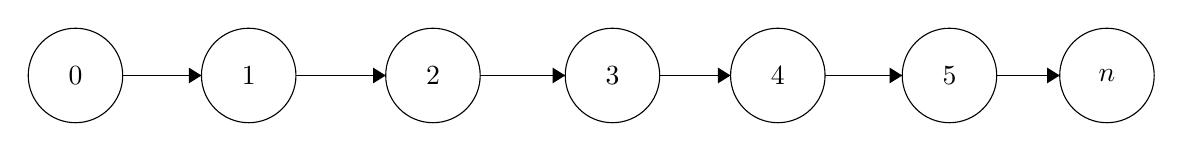
\begin{tikzpicture}[scale=0.2] \tikzstyle{every node}+=[inner sep=0pt] \draw [black] (17.5,-22.3) circle (3); \draw (17.5,-22.3) node {$1$}; \draw [black] (6.5,-22.3) circle (3); \draw (6.5,-22.3) node {$0$}; \draw [black] (29.2,-22.3) circle (3); \draw (29.2,-22.3) node {$2$}; \draw [black] (40.6,-22.3) circle (3); \draw (40.6,-22.3) node {$3$}; \draw [black] (51.1,-22.3) circle (3); \draw (51.1,-22.3) node {$4$}; \draw [black] (62,-22.3) circle (3); \draw (62,-22.3) node {$5$}; \draw [black] (72,-22.3) circle (3); \draw (72,-22.3) node {$n$}; \draw [black] (9.5,-22.3) -- (14.5,-22.3); \fill [black] (14.5,-22.3) -- (13.7,-21.8) -- (13.7,-22.8); \draw [black] (20.5,-22.3) -- (26.2,-22.3); \fill [black] (26.2,-22.3) -- (25.4,-21.8) -- (25.4,-22.8); \draw [black] (32.2,-22.3) -- (37.6,-22.3); \fill [black] (37.6,-22.3) -- (36.8,-21.8) -- (36.8,-22.8); \draw [black] (43.6,-22.3) -- (48.1,-22.3); \fill [black] (48.1,-22.3) -- (47.3,-21.8) -- (47.3,-22.8); \draw [black] (54.1,-22.3) -- (59,-22.3); \fill [black] (59,-22.3) -- (58.2,-21.8) -- (58.2,-22.8); \draw [black] (65,-22.3) -- (69,-22.3); \fill [black] (69,-22.3) -- (68.2,-21.8) -- (68.2,-22.8); \end{tikzpicture} \end{center}


\section{La logica K4DLZ}

la logica K4DLZ, detta anche logica $\Omega$ è la logica che ha,
oltre all'assioma K, i seguenti assiomi:
\begin{itemize}
\item 4: $\boa\implies\boxx{\boa}$ --> transitività
\item D: $\boa\implies\dia$ --> serialità
\item L: $\boxx{(a\wedge\boa\implies b)}\vee\boxx{(b\wedge\boxx b\implies a)}$
--> debole connessione
\item Z: $\boxx{(\boa\implies a)\implies(\diam{\boa}\implies\boa)}$
\end{itemize}
L'assioma Z, non ha alcuna interpretazione preso a se stante, ma in
combinazione con gli altri implica che tra due mondi connessi c'è
solo un numero finito di mondi, a due a due connessi.


\section{Correttezza di K4DLZ}

Ip) $\teolm{\Omega}a$

Ts) $\vera{(\omega,<)}a$\\


Per dimostrare questo teorema dobbiamo dimostrare che ogni teorema
di K4DLZ è una formula valida. Poiché ogni teorema di $\Omega$ è
una serie di applicazioni degli assiomi o delle regole di inferenza,
dobbiamo assicurare che:
\begin{enumerate}
\item Modus Ponens e la regola di necessitazione fanno passare da formule
valide a formule valide. Come abbiamo dimostrato, questo è sempre
vero.
\item Gli assiomi siano formule valide:\end{enumerate}
\begin{itemize}
\item A1, A2, A3, K sono validi su ogni frame, e quindi sono validi anche
su ($\omega$, <)
\item 4 è valido su ogni frame transitivo, e quindi è valido anche su ($\omega$,
<) essendo transitivo
\item D è valido su ogni frame seriale, e quindi è valido anche su ($\omega$,
<) essendo seriale.
\item L è valido su ogni frame debolmente connesso, e quindi è valido anche
su ($\omega$, <) essendo debolmente connesso.\\

\end{itemize}
Dobbiamo quindi dimostrare solo la validità di Z.

Z è l'assioma $\boxx{(\boa\implies a)\implies(\diam{\boa}\implies\boa)}$,
per dimostrare che è valido basta considerare il caso in cui gli antecedenti
delle implicazioni siano validi

supponiamo dunque che esistano due mondi $\alpha$ e $\beta$ con
$\alpha<\beta$ tali che

$\veraw{(\omega,\,<)}{\alpha}{\boxx{(\boa\implies a)}}$

$\veraw{(\omega,\,<)}{\alpha}{\diam{\boa}}$

$\veraw{(\omega,\,<)}{\beta}{\boa}$

allora da quest'ultima, viste le altre proprietà del frame, $\forall\eta>\beta$
avremo:

$\veraw{(\omega,\,<)}{\eta}a$

dalla prima invece abbiamo:

$\veraw{(\omega,\,<)}{\beta}{\boa\implies a}$

e allora, applicando il modus ponens

$\veraw{(\omega,\,<)}{\beta}a$

Ma, allora possiamo applicare lo stesso ragionamento per $\beta-1$,
poiché:

$\veraw{(\omega,\,<)}{\beta-1}{\boa}$

\begin{center} 
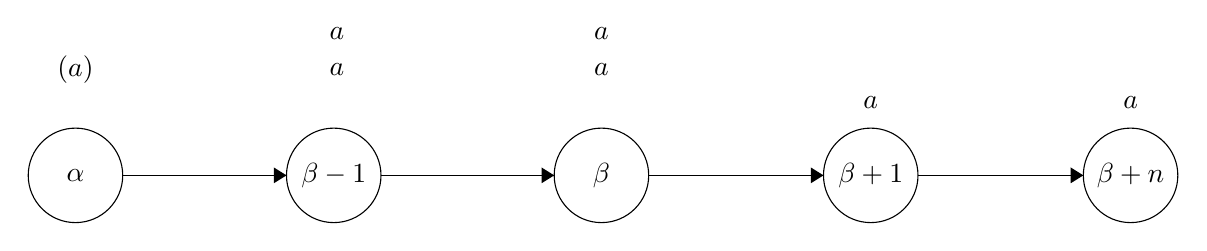
\begin{tikzpicture}[scale=0.2] 
\tikzstyle{every node}+=[inner sep=0pt] 
\draw [black] (6.1,-28.6) circle (3); 
\draw (6.1,-28.6) node {$\alpha$}; 
\draw [black] (22.5,-28.6) circle (3); 
\draw (22.5,-28.6) node {$\beta-1$}; 
\draw [black] (56.6,-28.6) circle (3); 
\draw (56.6,-28.6) node {$\beta+1$}; 
\draw [black] (73.1,-28.6) circle (3); 
\draw (73.1,-28.6) node {$\beta+n$}; 
\draw [black] (39.5,-28.6) circle (3); 
\draw (39.5,-28.6) node {$\beta$}; 
\draw (73.1,-24) node {$a$}; 
\draw (56.6,-24) node {$a$}; 
\draw (39.5,-24) node {$\boa$}; 
\draw (39.5,-21.9) node {$\boa\implies a$}; 
\draw (39.5,-19.6) node {$a$}; 
\draw (6.1,-24.6) node {$\diam{\boa}$}; 
\draw (6.1,-21.9) node {$\boxx{(\boa\implies a)}$}; 
\draw (22.5,-24) node {$\boa$}; 
\draw (22.7,-21.9) node {$\boa\implies a$}; 
\draw (22.7,-19.6) node {$a$}; 
\draw [black] (9.1,-28.6) -- (19.5,-28.6); 
\fill [black] (19.5,-28.6) -- (18.7,-28.1) -- (18.7,-29.1); 
\draw [black] (59.6,-28.6) -- (70.1,-28.6); 
\fill [black] (70.1,-28.6) -- (69.3,-28.1) -- (69.3,-29.1); 
\draw [black] (42.5,-28.6) -- (53.6,-28.6); 
\fill [black] (53.6,-28.6) -- (52.8,-28.1) -- (52.8,-29.1); 
\draw [black] (25.5,-28.6) -- (36.5,-28.6); 
\fill [black] (36.5,-28.6) -- (35.7,-28.1) -- (35.7,-29.1);
\end{tikzpicture} 
\end{center}

Ma, siccome esiste un numero finito di mondi tra $\alpha$ e $\beta$,
arriveremo a un certo punto a provare che:

$\veraw{(\omega,\,<)}{\alpha+1}a$

e quindi:

$\veraw{(\omega,\,<)}{\alpha}{\boa}$

\begin{center} 
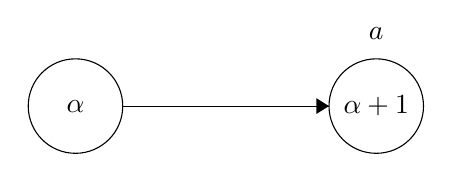
\begin{tikzpicture}[scale=0.2] 
\tikzstyle{every node}+=[inner sep=0pt] 
\draw [black] (28,-22.8) circle (3); 
\draw (28,-22.8) node {$\alpha$}; 
\draw [black] (47.1,-22.8) circle (3); 
\draw (47.1,-22.8) node {$\alpha+1$}; 
\draw (47.1,-18.2) node {$a$}; 
\draw (27.9,-18.6) node {$\boa$}; 
\draw [black] (31,-22.8) -- (44.1,-22.8); 
\fill [black] (44.1,-22.8) -- (43.3,-22.3) -- (43.3,-23.3); 
\end{tikzpicture} 
\end{center}

e la tesi è dimostrata.


\section{Completezza di K4DLZ}

Ip) $\vera{(\omega,<)}a$

Ts)$\teolm{\Omega}a$ \\


Questa dimostrazione è così lunga da essere suddivisa per convenienza
in punti

\textbf{1)}

Per assurdo supponiamo che non valga la tesi, cioè che 

$\nonTeor{\Omega}a$, per il lemma di verità si ha anche $\nonvera{M^{\Omega}}a$,
$M^{\Omega}=M_{1}$

$M_{1}$è seriale, transitivo e debolmente connesso, infatti queste
proprietà si conservano quando si passa dalla logica al modello canonico.

Dato che $\nonvera{M^{\Omega}}a$, in particolare esiste un mondo
$\alpha$ in cui $\nonveraw{M_{1}}{\alpha}a$

\textbf{2)}

$M_{2}=M_{1}^{\alpha}$, dove $M_{1}^{\alpha}$ è il sottomodello
generato da $\alpha$.

$M_{2}$ è seriale, transitivo e connesso. La serialità e la transitività
vengono direttamente da $M_{1}$, esaminiamo la connessione.

$M_{2}=(S_{2},R_{2},V_{2})$ se $\delta\in S_{2}$e $\gamma\in S_{2}$
allora $(\alpha,\gamma)\in R_{1}^{*}$ e $(\alpha,\delta)\in R_{1}^{*}$

Dato che $R_{1}$è già transitiva(vedi punto 1) la sua chiusura riflessiva
e transitiva si limita a unire la relazione identica (cioè aggiunge
gli autoanelli ai mondi)

Dal momento che $R_{1}$ è debolmente connessa, $R_{1}$, avendo anche
la riflessività è connessa.

Inoltre $\nonvera{M_{2}}a$, infatti sappiamo che se $\vera Ma$ allora
$\vera{M^{\alpha}}a$ per ogni mondo $\alpha$ di $M$

\textbf{3)}

$M^{3}=$$\Gamma$-filtrazione di $M_{2}$, con $\Gamma=Stf(a)$

dove come $\Gamma$-filtrazione delle relazione di raggiungibilità
di $M_{2}$ si prende la filtrazione transitiva. 

$M^{3}$ è ancora seriale e connesso ed è transitivo per costruzione,
inoltre il suo insieme di mondi ha cardinalità limitata superiormente
da $2^{|Sfm(A)|}$

Inoltre $\nonvera{M_{3}}a$

\textbf{4-pre)}

Diciamo palloncino un frame $(T,\rho)$ dove 

$T=\{\alpha_{1},\alpha_{2},...,\alpha_{n},\alpha_{n+1},...,\alpha_{n+m}\}$
e 

$i.j\in\rho\ \iff\ i<j\ oppure\ i,j\geq n$ 

Sostanzialmente il grafo di $\rho$ si presenta nella seguente forma
(a meno degli archi che esprimono il fatto che $\rho$ è transitiva).\\


\begin{center} 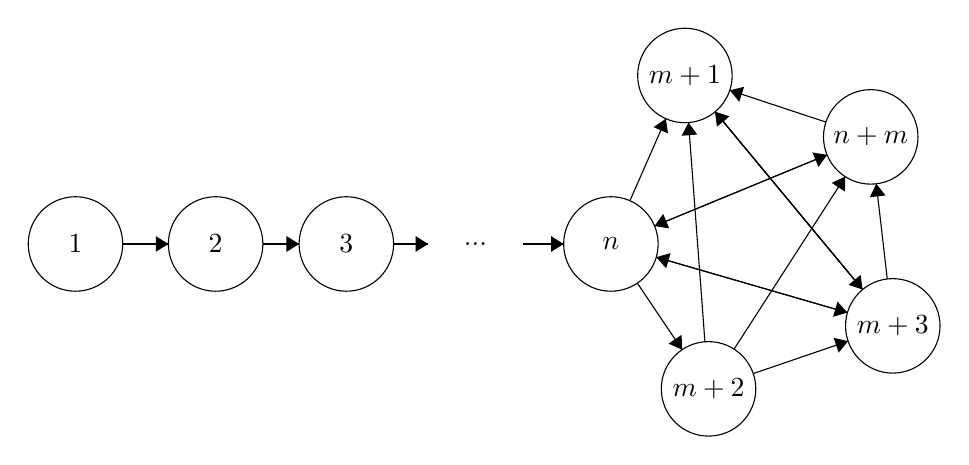
\begin{tikzpicture}[scale=0.2] \tikzstyle{every node}+=[inner sep=0pt] \draw [black] (5.5,-30.4) circle (3); \draw (5.5,-30.4) node {$1$}; \draw [black] (14.4,-30.4) circle (3); \draw (14.4,-30.4) node {$2$}; \draw [black] (22.7,-30.4) circle (3); \draw (22.7,-30.4) node {$3$}; \draw [black] (39.5,-30.4) circle (3); \draw (39.5,-30.4) node {$n$}; \draw [black] (44.2,-19.7) circle (3); \draw (44.2,-19.7) node {$m+1$}; \draw [black] (45.7,-39.6) circle (3); \draw (45.7,-39.6) node {$m+2$}; \draw [black] (57.4,-35.6) circle (3); \draw (57.4,-35.6) node {$m+3$}; \draw [black] (56,-23.6) circle (3); \draw (56,-23.6) node {$n+m$};
\draw (30.9,-30.4) node {$...$}; \draw [black] (8.5,-30.4) -- (11.4,-30.4); \fill [black] (11.4,-30.4) -- (10.6,-29.9) -- (10.6,-30.9); \draw [black] (17.4,-30.4) -- (19.7,-30.4); \fill [black] (19.7,-30.4) -- (18.9,-29.9) -- (18.9,-30.9); \draw [black] (40.71,-27.65) -- (42.99,-22.45); \fill [black] (42.99,-22.45) -- (42.21,-22.98) -- (43.13,-23.38); \draw [black] (42.27,-29.26) -- (53.23,-24.74); \fill [black] (53.23,-24.74) -- (52.3,-24.59) -- (52.68,-25.51); \draw [black] (42.38,-31.24) -- (54.52,-34.76); \fill [black] (54.52,-34.76) -- (53.89,-34.06) -- (53.61,-35.02); \draw [black] (41.18,-32.89) -- (44.02,-37.11); \fill [black] (44.02,-37.11) -- (43.99,-36.17) -- (43.16,-36.73); \draw [black] (48.54,-38.63) -- (54.56,-36.57); \fill [black] (54.56,-36.57) -- (53.64,-36.36) -- (53.97,-37.3); \draw [black] (57.05,-32.62) -- (56.35,-26.58); \fill [black] (56.35,-26.58) -- (55.94,-27.43) -- (56.94,-27.32); \draw [black] (53.15,-22.66) -- (47.05,-20.64); \fill [black] (47.05,-20.64) -- (47.65,-21.37) -- (47.96,-20.42); \draw [black] (55.48,-33.29) -- (46.12,-22.01); \fill [black] (46.12,-22.01) -- (46.24,-22.94) -- (47.01,-22.3); \draw [black] (54.52,-34.76) -- (42.38,-31.24); \fill [black] (42.38,-31.24) -- (43.01,-31.94) -- (43.29,-30.98); \draw [black] (47.32,-37.08) -- (54.38,-26.12); \fill [black] (54.38,-26.12) -- (53.52,-26.52) -- (54.36,-27.07); \draw [black] (45.47,-36.61) -- (44.43,-22.69); \fill [black] (44.43,-22.69) -- (43.99,-23.53) -- (44.98,-23.45); \draw [black] (55.48,-33.29) -- (46.12,-22.01); \fill [black] (46.12,-22.01) -- (46.24,-22.94) -- (47.01,-22.3); \draw [black] (46.12,-22.01) -- (55.48,-33.29); \fill [black] (55.48,-33.29) -- (55.36,-32.36) -- (54.59,-33); \draw [black] (53.23,-24.74) -- (42.27,-29.26); \fill [black] (42.27,-29.26) -- (43.2,-29.41) -- (42.82,-28.49); \draw [black] (25.7,-30.4) -- (27.9,-30.4); \fill [black] (27.9,-30.4) -- (27.1,-29.9) -- (27.1,-30.9); \draw [black] (33.9,-30.4) -- (36.5,-30.4); \fill [black] (36.5,-30.4) -- (35.7,-29.9) -- (35.7,-30.9); \end{tikzpicture} \end{center}

\textbf{4)}

Si vuole trovare un modello a palloncino $P$ che sia modello di $\Omega$,
in cui $\nonvera Pa$, e tale che $P$ abbia tutte le proprietà di
$M_{3}$ 

$M_{3}$ potrebbe presentare dei ``grovigli'' di questo tipo:

\begin{center} 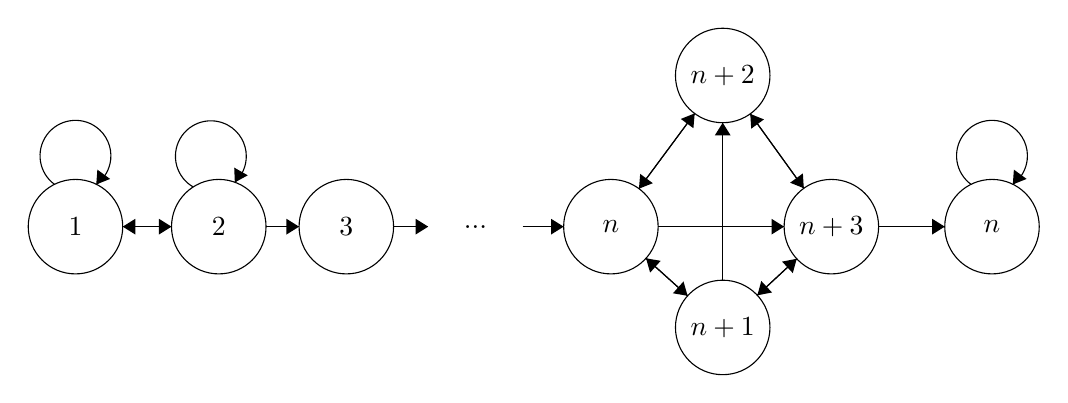
\begin{tikzpicture}[scale=0.2] \tikzstyle{every node}+=[inner sep=0pt] \draw [black] (5.5,-30.4) circle (3); \draw (5.5,-30.4) node {$1$}; \draw [black] (14.6,-30.4) circle (3); \draw (14.6,-30.4) node {$2$}; \draw [black] (22.7,-30.4) circle (3); \draw (22.7,-30.4) node {$3$}; \draw [black] (39.5,-30.4) circle (3); \draw (39.5,-30.4) node {$n$}; \draw [black] (46.6,-20.8) circle (3); \draw (46.6,-20.8) node {$n+2$}; \draw [black] (46.6,-36.8) circle (3); \draw (46.6,-36.8) node {$n+1$};
\draw (30.9,-30.4) node {$...$}; \draw [black] (53.5,-30.4) circle (3); \draw (53.5,-30.4) node {$n+3$}; \draw [black] (63.7,-30.4) circle (3); \draw (63.7,-30.4) node {$n$}; \draw [black] (8.5,-30.4) -- (11.6,-30.4); \fill [black] (11.6,-30.4) -- (10.8,-29.9) -- (10.8,-30.9); \draw [black] (17.6,-30.4) -- (19.7,-30.4); \fill [black] (19.7,-30.4) -- (18.9,-29.9) -- (18.9,-30.9); \draw [black] (41.28,-27.99) -- (44.82,-23.21); \fill [black] (44.82,-23.21) -- (43.94,-23.56) -- (44.74,-24.15); \draw [black] (41.73,-32.41) -- (44.37,-34.79); \fill [black] (44.37,-34.79) -- (44.11,-33.88) -- (43.44,-34.63); \draw [black] (46.6,-33.8) -- (46.6,-23.8); \fill [black] (46.6,-23.8) -- (46.1,-24.6) -- (47.1,-24.6); \draw [black] (25.7,-30.4) -- (27.9,-30.4); \fill [black] (27.9,-30.4) -- (27.1,-29.9) -- (27.1,-30.9); \draw [black] (33.9,-30.4) -- (36.5,-30.4); \fill [black] (36.5,-30.4) -- (35.7,-29.9) -- (35.7,-30.9); \draw [black] (4.177,-27.72) arc (234:-54:2.25); \fill [black] (6.82,-27.72) -- (7.7,-27.37) -- (6.89,-26.78); \draw [black] (12.987,-27.885) arc (240.4087:-47.5913:2.25); \fill [black] (15.62,-27.59) -- (16.44,-27.14) -- (15.58,-26.65); \draw [black] (11.6,-30.4) -- (8.5,-30.4); \fill [black] (8.5,-30.4) -- (9.3,-30.9) -- (9.3,-29.9); \draw [black] (42.5,-30.4) -- (50.5,-30.4); \fill [black] (50.5,-30.4) -- (49.7,-29.9) -- (49.7,-30.9); \draw [black] (56.5,-30.4) -- (60.7,-30.4); \fill [black] (60.7,-30.4) -- (59.9,-29.9) -- (59.9,-30.9); \draw [black] (62.377,-27.72) arc (234:-54:2.25); \fill [black] (65.02,-27.72) -- (65.9,-27.37) -- (65.09,-26.78); \draw [black] (48.8,-34.76) -- (51.3,-32.44); \fill [black] (51.3,-32.44) -- (50.37,-32.62) -- (51.05,-33.35); \draw [black] (51.75,-27.96) -- (48.35,-23.24); \fill [black] (48.35,-23.24) -- (48.41,-24.18) -- (49.22,-23.59); \draw [black] (48.35,-23.24) -- (51.75,-27.96); \fill [black] (51.75,-27.96) -- (51.69,-27.02) -- (50.88,-27.61); \draw [black] (51.3,-32.44) -- (48.8,-34.76); \fill [black] (48.8,-34.76) -- (49.73,-34.58) -- (49.05,-33.85); \draw [black] (44.37,-34.79) -- (41.73,-32.41); \fill [black] (41.73,-32.41) -- (41.99,-33.32) -- (42.66,-32.57); \draw [black] (44.82,-23.21) -- (41.28,-27.99); \fill [black] (41.28,-27.99) -- (42.16,-27.64) -- (41.36,-27.05); \end{tikzpicture} \end{center}

L'idea di questo punto 4 è ``sciogliere'' questi grovigli.

Sia $M_{3}=(S,R,V)$, introduciamo una relazione $\approx\subseteq S\times S$

$\alpha\approx\beta$ se e solo se: $(\alpha R\beta)\ e\ (\beta R\alpha)\ oppure\ \alpha=\beta$

$\approx$è una relazione di equivalenza infatti:

è riflessiva per costruzione 

è simmetrica infatti: $\alpha\approx\beta$ $(\alpha\neq\beta)$se
e solo se: $(\alpha R\beta)\ e\ (\beta R\alpha)$ se e solo se $\beta\approx\alpha$

è transitiva infatti: $\alpha\approx\beta$, \foreignlanguage{english}{$\beta\approx\gamma$
}se e solo se: $(\alpha R\beta)\ e\ (\beta R\alpha)$ e $(\gamma R\beta)\ e\ (\beta R\gamma)$,
per la transitività di $R$ si ha anche $(\alpha R\gamma),\ (\gamma R\alpha)$
da cui: $\alpha\approx\gamma$

Per questi motivi $\approx$è una relazione d'equivalenza, e come
tale partiziona l'insieme $S$ e ne definisce un insieme quoziente
$S/\approx$

Chiamiamo R-cluster la classe di equivalenza$C_{\alpha}$ di $\alpha$,
e definiamo in modo abbastanza naturale la relazione di $\leq$nel
modo seguente:

$C_{\alpha}\leq C_{\beta}$ se e solo se: $\alpha R\beta$ oppure
$C_{\alpha}=C_{\beta}$

$C_{\alpha}<C_{\beta}$ se e solo se: $\alpha R\beta$ e $C_{\alpha}\neq C_{\beta}$ 

\begin{center} 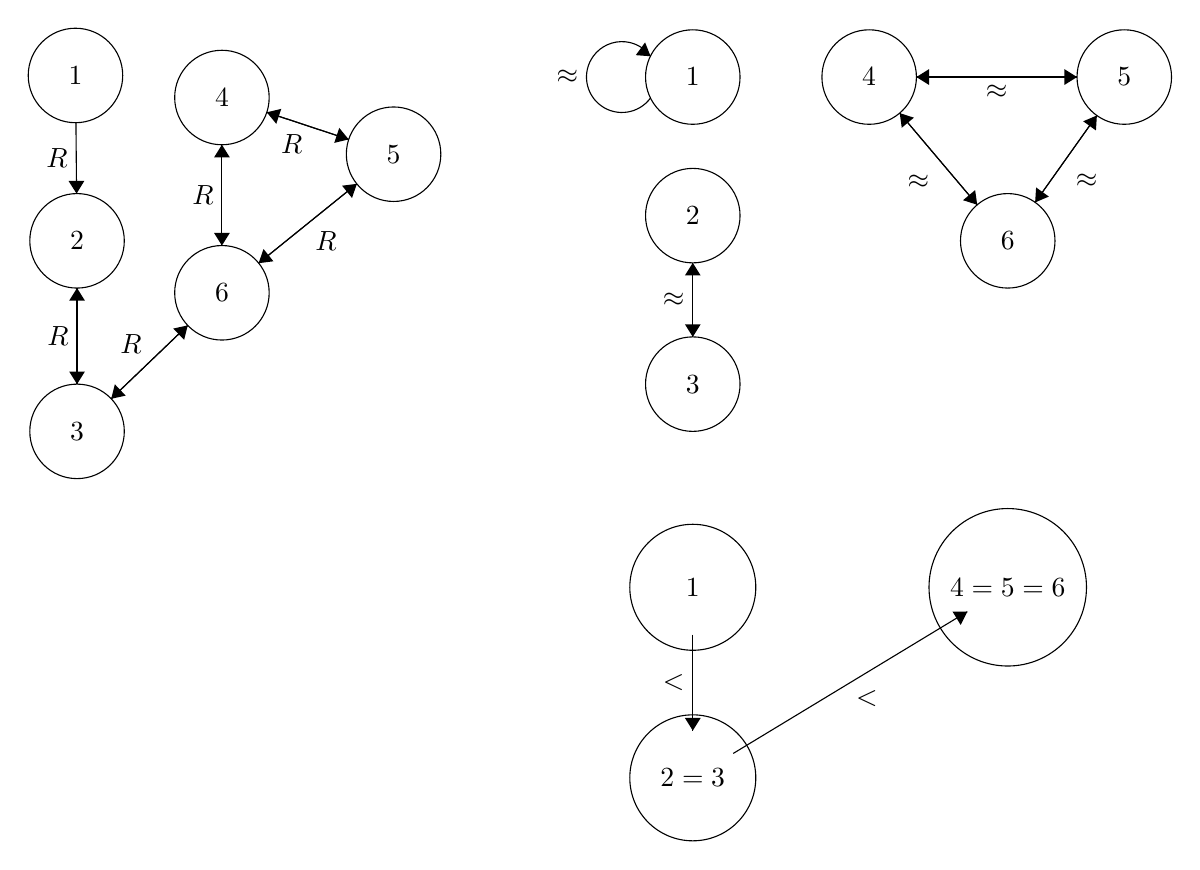
\begin{tikzpicture}[scale=0.2] \tikzstyle{every node}+=[inner sep=0pt] \draw [black] (5.1,-5.6) circle (3); \draw (5.1,-5.6) node {$1$}; \draw [black] (5.2,-16.1) circle (3); \draw (5.2,-16.1) node {$2$}; \draw [black] (5.2,-28.2) circle (3); \draw (5.2,-28.2) node {$3$}; \draw [black] (14.4,-7) circle (3); \draw (14.4,-7) node {$4$}; \draw [black] (25.3,-10.6) circle (3); \draw (25.3,-10.6) node {$5$}; \draw [black] (14.4,-19.4) circle (3); \draw (14.4,-19.4) node {$6$}; \draw [black] (44.3,-5.7) circle (3); \draw (44.3,-5.7) node {$1$}; \draw [black] (44.3,-14.5) circle (3); \draw (44.3,-14.5) node {$2$}; \draw [black] (44.3,-25.2) circle (3); \draw (44.3,-25.2) node {$3$}; \draw [black] (55.5,-5.7) circle (3); \draw (55.5,-5.7) node {$4$}; \draw [black] (71.7,-5.7) circle (3); \draw (71.7,-5.7) node {$5$}; \draw [black] (64.3,-16.1) circle (3); \draw (64.3,-16.1) node {$6$}; \draw [black] (44.3,-38.1) circle (4); \draw (44.3,-38.1) node {$1$}; \draw [black] (44.3,-50.2) circle (4); \draw (44.3,-50.2) node {$2=3$}; \draw [black] (64.3,-38.1) circle (5); \draw (64.3,-38.1) node {$4=5=6$}; \draw [black] (5.13,-8.6) -- (5.17,-13.1); \fill [black] (5.17,-13.1) -- (5.66,-12.3) -- (4.66,-12.3); \draw (4.64,-10.85) node [left] {$R$}; \draw [black] (5.2,-19.1) -- (5.2,-25.2); \fill [black] (5.2,-25.2) -- (5.7,-24.4) -- (4.7,-24.4); \draw (4.7,-22.15) node [left] {$R$}; \draw [black] (5.2,-25.2) -- (5.2,-19.1); \fill [black] (5.2,-19.1) -- (4.7,-19.9) -- (5.7,-19.9); \draw [black] (7.37,-26.13) -- (12.23,-21.47); \fill [black] (12.23,-21.47) -- (11.31,-21.67) -- (12,-22.39); \draw [black] (14.4,-10) -- (14.4,-16.4); \fill [black] (14.4,-16.4) -- (14.9,-15.6) -- (13.9,-15.6); \draw (13.9,-13.2) node [left] {$R$}; \draw [black] (14.4,-16.4) -- (14.4,-10); \fill [black] (14.4,-10) -- (13.9,-10.8) -- (14.9,-10.8); \draw [black] (17.25,-7.94) -- (22.45,-9.66); \fill [black] (22.45,-9.66) -- (21.85,-8.93) -- (21.53,-9.88); \draw (18.83,-9.34) node [below] {$R$}; \draw [black] (22.45,-9.66) -- (17.25,-7.94); \fill [black] (17.25,-7.94) -- (17.85,-8.67) -- (18.17,-7.72); \draw [black] (22.97,-12.48) -- (16.73,-17.52); \fill [black] (16.73,-17.52) -- (17.67,-17.4) -- (17.04,-16.62); \draw [black] (16.73,-17.52) -- (22.97,-12.48); \fill [black] (22.97,-12.48) -- (22.03,-12.6) -- (22.66,-13.38); \draw (21.01,-15.49) node [below] {$R$}; \draw [black] (12.23,-21.47) -- (7.37,-26.13); \fill [black] (7.37,-26.13) -- (8.29,-25.93) -- (7.6,-25.21); \draw (8.63,-23.32) node [above] {$R$}; \draw [black] (44.3,-17.5) -- (44.3,-22.2); \fill [black] (44.3,-22.2) -- (44.8,-21.4) -- (43.8,-21.4); \draw (43.8,-19.85) node [left] {$\approx$}; \draw [black] (44.3,-22.2) -- (44.3,-17.5); \fill [black] (44.3,-17.5) -- (43.8,-18.3) -- (44.8,-18.3); \draw [black] (58.5,-5.7) -- (68.7,-5.7); \fill [black] (68.7,-5.7) -- (67.9,-5.2) -- (67.9,-6.2); \draw (63.6,-6.2) node [below] {$\approx$}; \draw [black] (68.7,-5.7) -- (58.5,-5.7); \fill [black] (58.5,-5.7) -- (59.3,-6.2) -- (59.3,-5.2); \draw [black] (57.44,-7.99) -- (62.36,-13.81); \fill [black] (62.36,-13.81) -- (62.23,-12.88) -- (61.46,-13.52); \draw (59.35,-12.34) node [left] {$\approx$}; \draw [black] (66.04,-13.66) -- (69.96,-8.14); \fill [black] (69.96,-8.14) -- (69.09,-8.51) -- (69.9,-9.09); \draw (68.59,-12.27) node [right] {$\approx$}; \draw [black] (69.96,-8.14) -- (66.04,-13.66); \fill [black] (66.04,-13.66) -- (66.91,-13.29) -- (66.1,-12.71); \draw [black] (62.36,-13.81) -- (57.44,-7.99); \fill [black] (57.44,-7.99) -- (57.57,-8.92) -- (58.34,-8.28); \draw [black] (41.62,-7.023) arc (-36:-324:2.25); \draw (37.05,-5.7) node [left] {$\approx$}; \fill [black] (41.62,-4.38) -- (41.27,-3.5) -- (40.68,-4.31); \draw [black] (44.3,-41.1) -- (44.3,-47.2); 
\fill [black] (44.3,-47.2) -- (44.8,-46.4) -- (43.8,-46.4); \draw (43.8,-44.15) node [left] {$<$}; \draw [black] (46.87,-48.65) -- (61.73,-39.65); \fill [black] (61.73,-39.65) -- (60.79,-39.64) -- (61.31,-40.49); \draw (55.35,-44.65) node [below] {$<$};
\end{tikzpicture} \end{center}

Se un R-cluster C contiene più di un elemento, la relazione R è riflessiva
su $C$ e si ha $C\leq C$, infatti detti $\alpha$ e $\beta$ due
elementi di $C$ si ha $\alpha R\beta$ e $\beta R\alpha$ quindi,
per la transitività di $R$ $\alpha R\alpha$,

inoltre $C=$$C_{\alpha}\leq C\alpha$ $=C$.

Se non è $C\leq C$, l’R-cluster $C$ si dice degenere ed è formato
da un unico elemento $\alpha$ per il quale non risulta $\alpha R\alpha$ 

Un palloncino può essere visto come una sequenza finita di cluster
di cui solo l’ultimo è non degenere. Ma nel nostro modello possono
esserci, oltre all’ultimo R-cluster $C_{\alpha}$, altri R-cluster
non degeneri.

Per ricondurmi a un palloncino, a partire da $M_{3}$ considero la
relazione $R'$ che ordina in modo arbitrario i mondi appartenenti
a uno stesso R-cluster che non sia l'ultimo.

$R'$ è così definita:
\begin{itemize}
\item Se$\alpha,\beta$ appartengono a cluster diversi allora $(\alpha,\beta)\in R'$se
e solo se $(\alpha,\beta)\in R$
\item Se $\alpha,\beta$ appartengono all'ultimo cluster $(\alpha,\beta)\in R'$
\item Se $\alpha,\beta$ appartengono allo stesso cluster, e non è l'ultimo,
detti $\gamma_{1},\gamma_{2},\dots,\gamma_{n}$, si pone $\gamma_{i}R'\gamma_{j}$
se e solo se $i<j$.
\item $(\alpha,\alpha)\notin R'$ (tolgo gli autoanelli)
\end{itemize}
A questo punto abbiamo un palloncino$P$ costruito su $S$,$R'$,
$V$, ed è lecito chiedersi se $\vera{M_{3}}a$ se e solo se $\vera Pa$.

Questo è ovviamente vero se $a$ non presenta connettivi modali.

Supponiamo allora che $a$ sia del tipo $\boxx d$.

Dato che$R'\subseteq R$,\\
\begin{center} 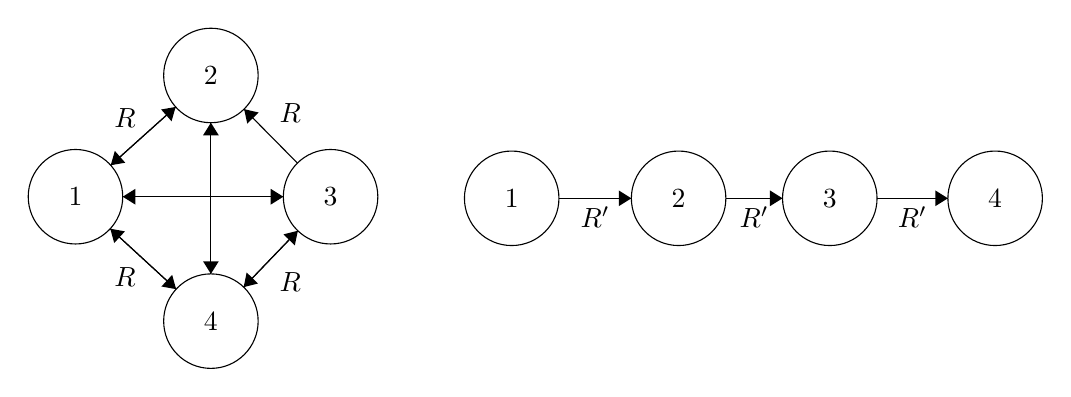
\begin{tikzpicture}[scale=0.2] \tikzstyle{every node}+=[inner sep=0pt] \draw [black] (11,-13.3) circle (3); \draw (11,-13.3) node {$1$}; \draw [black] (19.6,-5.6) circle (3); \draw (19.6,-5.6) node {$2$}; \draw [black] (27.2,-13.3) circle (3); \draw (27.2,-13.3) node {$3$}; \draw [black] (19.6,-21.2) circle (3); \draw (19.6,-21.2) node {$4$}; \draw [black] (38.7,-13.4) circle (3); \draw (38.7,-13.4) node {$1$}; \draw [black] (49.3,-13.4) circle (3); \draw (49.3,-13.4) node {$2$}; \draw [black] (58.9,-13.4) circle (3); \draw (58.9,-13.4) node {$3$}; \draw [black] (69.4,-13.4) circle (3); \draw (69.4,-13.4) node {$4$}; \draw [black] (13.24,-11.3) -- (17.36,-7.6); \fill [black] (17.36,-7.6) -- (16.44,-7.76) -- (17.1,-8.51); \draw [black] (17.36,-7.6) -- (13.24,-11.3); \fill [black] (13.24,-11.3) -- (14.16,-11.14) -- (13.5,-10.39); \draw (14.14,-8.96) node [above] {$R$}; \draw [black] (25.09,-11.16) -- (21.71,-7.74); \fill [black] (21.71,-7.74) -- (21.91,-8.66) -- (22.63,-7.95); \draw (23.93,-7.98) node [right] {$R$}; \draw [black] (17.39,-19.17) -- (13.21,-15.33); \fill [black] (13.21,-15.33) -- (13.46,-16.24) -- (14.14,-15.5); \draw (14.14,-17.74) node [below] {$R$}; \draw [black] (13.21,-15.33) -- (17.39,-19.17); \fill [black] (17.39,-19.17) -- (17.14,-18.26) -- (16.46,-19); \draw [black] (21.68,-19.04) -- (25.12,-15.46); \fill [black] (25.12,-15.46) -- (24.21,-15.69) -- (24.93,-16.39); \draw (23.93,-18.72) node [right] {$R$}; \draw [black] (25.12,-15.46) -- (21.68,-19.04); \fill [black] (21.68,-19.04) -- (22.59,-18.81) -- (21.87,-18.11); \draw [black] (19.6,-8.6) -- (19.6,-18.2); \fill [black] (19.6,-18.2) -- (20.1,-17.4) -- (19.1,-17.4); \draw [black] (19.6,-18.2) -- (19.6,-8.6); \fill [black] (19.6,-8.6) -- (19.1,-9.4) -- (20.1,-9.4); \draw [black] (24.2,-13.3) -- (14,-13.3); \fill [black] (14,-13.3) -- (14.8,-13.8) -- (14.8,-12.8); \draw [black] (14,-13.3) -- (24.2,-13.3); \fill [black] (24.2,-13.3) -- (23.4,-12.8) -- (23.4,-13.8); \draw [black] (41.7,-13.4) -- (46.3,-13.4); \fill [black] (46.3,-13.4) -- (45.5,-12.9) -- (45.5,-13.9); \draw (44,-13.9) node [below] {$R'$}; \draw [black] (52.3,-13.4) -- (55.9,-13.4); \fill [black] (55.9,-13.4) -- (55.1,-12.9) -- (55.1,-13.9); \draw (54.1,-13.9) node [below] {$R'$}; \draw [black] (61.9,-13.4) -- (66.4,-13.4); \fill [black] (66.4,-13.4) -- (65.6,-12.9) -- (65.6,-13.9); \draw (64.15,-13.9) node [below] {$R'$}; \end{tikzpicture} \end{center} 

se $\boxx d$ è vera in un mondo $\beta$ di $M_{3}$, $\boxx d$
è vera anche nel mondo $\beta$ di $M\lyxmathsym{’}$ ($R'$ ha
meno archi quindi è più facile per $\boxx x$ essere soddisfatta)

Sia allora $\boxx d$ vera in un mondo $\beta$ di $M\lyxmathsym{’}$
e supponiamo che $\boxx d$ non sia vera nel mondo $\beta$ di $M_{3}$.

Se è così, $d$ dovrà allora risultare falsa in un mondo $\gamma$
tale che $(\beta,\gamma)\in R$ mentre $(\beta,\gamma)\notin R\lyxmathsym{’}$.

\begin{center} 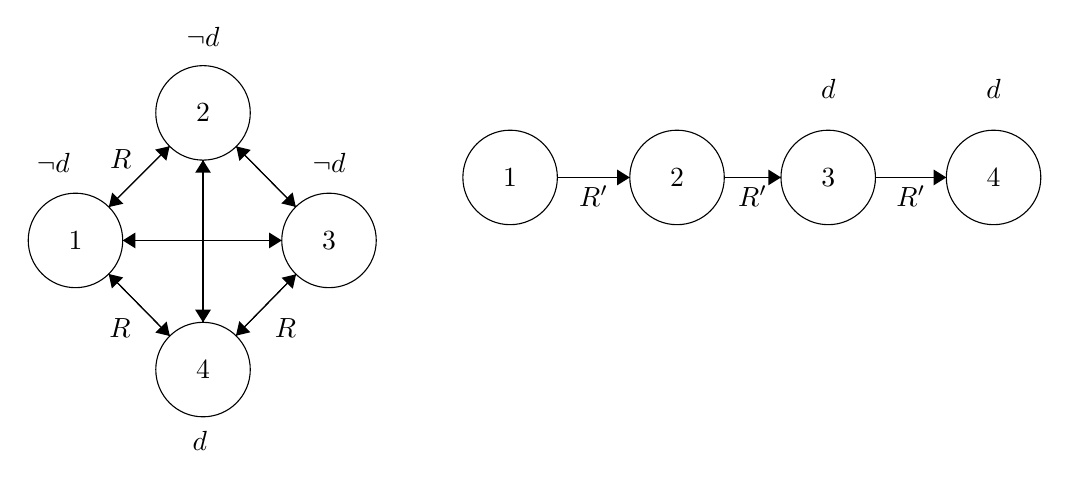
\begin{tikzpicture}[scale=0.2] \tikzstyle{every node}+=[inner sep=0pt] \draw [black] (11.1,-17.4) circle (3); \draw (11.1,-17.4) node {$1$}; \draw [black] (19.2,-9.3) circle (3); \draw (19.2,-9.3) node {$2$}; \draw [black] (27.2,-17.4) circle (3); \draw (27.2,-17.4) node {$3$}; \draw [black] (19.2,-25.6) circle (3); \draw (19.2,-25.6) node {$4$}; \draw [black] (38.7,-13.4) circle (3); \draw (38.7,-13.4) node {$1$}; \draw [black] (49.3,-13.4) circle (3); \draw (49.3,-13.4) node {$2$}; \draw [black] (58.9,-13.4) circle (3); \draw (58.9,-13.4) node {$3$}; \draw [black] (69.4,-13.4) circle (3); \draw (69.4,-13.4) node {$4$};
\draw (27.2,-12.5) node {$\neg\boxx d$};
\draw (19.2,-4.5) node {$\neg d$};
\draw (9.7,-12.5) node {$\neg d$};
\draw (19,-30.1) node {$d$};
\draw (58.9,-7.8) node {$\boxx d$};
\draw (69.4,-7.8) node {$d$}; 
\draw [black] (13.22,-15.28) -- (17.08,-11.42); 
\fill [black] (17.08,-11.42) -- (16.16,-11.63) -- (16.87,-12.34); \draw [black] (17.08,-11.42) -- (13.22,-15.28); 
\fill [black] (13.22,-15.28) -- (14.14,-15.07) -- (13.43,-14.36); \draw (13.98,-12.87) node [above] {$R$}; 
\draw [black] (25.09,-15.27) -- (21.31,-11.43); \fill [black] (21.31,-11.43) -- (21.51,-12.35) -- (22.23,-11.65);
\draw [black] (17.09,-23.47) -- (13.21,-19.53); \fill [black] (13.21,-19.53) -- (13.41,-20.45) -- (14.13,-19.75); 
\draw (14.63,-22.97) node [left] {$R$}; \draw [black] (13.21,-19.53) -- (17.09,-23.47); \fill [black] (17.09,-23.47) -- (16.89,-22.55) -- (16.17,-23.25); \draw [black] (21.29,-23.45) -- (25.11,-19.55); \fill [black] (25.11,-19.55) -- (24.19,-19.77) -- (24.9,-20.47); 
\draw (23.73,-22.97) node [right] {$R$}; \draw [black] (25.11,-19.55) -- (21.29,-23.45); \fill [black] (21.29,-23.45) -- (22.21,-23.23) -- (21.5,-22.53); \draw [black] (19.2,-12.3) -- (19.2,-22.6); \fill [black] (19.2,-22.6) -- (19.7,-21.8) -- (18.7,-21.8); \draw [black] (19.2,-22.6) -- (19.2,-12.3); \fill [black] (19.2,-12.3) -- (18.7,-13.1) -- (19.7,-13.1); \draw [black] (24.2,-17.4) -- (14.1,-17.4); \fill [black] (14.1,-17.4) -- (14.9,-17.9) -- (14.9,-16.9); \draw [black] (14.1,-17.4) -- (24.2,-17.4); \fill [black] (24.2,-17.4) -- (23.4,-16.9) -- (23.4,-17.9); \draw [black] (41.7,-13.4) -- (46.3,-13.4); \fill [black] (46.3,-13.4) -- (45.5,-12.9) -- (45.5,-13.9); \draw (44,-13.9) node [below] {$R'$}; \draw [black] (52.3,-13.4) -- (55.9,-13.4); \fill [black] (55.9,-13.4) -- (55.1,-12.9) -- (55.1,-13.9); \draw (54.1,-13.9) node [below] {$R'$}; \draw [black] (61.9,-13.4) -- (66.4,-13.4); \fill [black] (66.4,-13.4) -- (65.6,-12.9) -- (65.6,-13.9); \draw (64.15,-13.9) node [below] {$R'$}; \draw [black] (21.31,-11.43) -- (25.09,-15.27); \fill [black] (25.09,-15.27) -- (24.89,-14.35) -- (24.17,-15.05); \end{tikzpicture} \end{center} 

Ovviamente se $(\beta,\gamma)\in R$ ma $(\beta,\gamma)\notin R\lyxmathsym{’}$,
i mondi $\beta,\gamma$ devono appartenere ad uno stesso R- cluster
che non è l’ultimo. (infatti se $(\beta,\gamma)\in R$ allora sono
nello stesso cluster, che viene ``sciolto'' in R')

Si può ora far uso dello Z-lemma che garantisce l’esistenza di un
mondo $\delta$ in un R- cluster $C_{\delta}$ tale che $C_{\beta}<C_{\delta}$
in cui $d$ non è vera (lo Z-lemma sarà enunciato e dimostrato nel
seguito).

Ma $C_{\beta}<C_{\delta}$ implica $(\beta,\delta)\in R\lyxmathsym{’}$
e dunque $\boxx d$ non sarebbe vera nel mondo $\beta$ del modello
M’, contro la nostra supposizione.

Dunque avendo dimostrato nel passo 3 che $a$ non è vera nel mondo
$\alpha$ del modello $M_{3}$, abbiamo che $a$ non è vera nel mondo
$\alpha$ del modello $M\lyxmathsym{’}$, costruito su un palloncino
e quindi $a$ non è valida su ogni palloncino.

\textbf{5) }Esiste un p-morfismo suriettivo da $(\omega,<)$ a un
palloncino P.

Sia P : $(T,\rho)$ dove 

$T=\{\alpha_{1},\alpha_{2},...,\alpha_{n},\alpha_{n+1},...,\alpha_{n+m}\}$
e 

$i.j\in\rho\ \iff\ i<j\ oppure\ i,j\geq n$ 

L'idea è di fare un p-morfismo la cui funzione f : manda i primi $n$
mondi di $\omega$ nel ``gambo'' e i mondi da $n+1$ in poi nella
parte ``tonda'' del palloncino contando modulo $m$.

Pertanto definiamo $f\ :\ \omega\rightarrow T$ (ricordando che i
mondi sono numerati, sia in $\omega$ che in $T$)

$f(i)=i\ se$$i\leq m+n$

$f(n+m+j)=n+((m+j)\ mod\ 4)$

$f$ è suriettiva (tutto il codominio $T$ è raggiunto)

Infatti ogni elemento $i\in T$ ha almeno controimmagine $i\in\omega$
(gli elementi nella parte ``tonda'' del palloncino ne avranno altre)

\framebox{\begin{minipage}[t]{1\columnwidth}%
Proprietà di un p-morfismo

1) $(\alpha,\,\beta)\in R_{1}\implies(f(\alpha),\, f(\beta))\in R_{2}$

2) $(f(\alpha),\,\eta)\in R_{2}\implies\exists\beta\in S_{1}\,:\, f(\beta)=\eta\,\wedge\,(\alpha,\,\beta)\in R_{1}$%
\end{minipage}}

1) Se $\alpha,\beta<n$ si ha banalmente $f(\alpha),f(\beta)$ per
come è definita $f$ ;

Se$f(\alpha),f(\beta)$ sono nella parte ``tonda'' la 1) vale perché
$f(\alpha),f(\beta)$ in relazione di equivalenza

Se $\alpha$ nel gambo e $\beta$ nella parte ``tonda'', comunque
vale la 1) ricordando la transitività di $\rho$

2) Se $f(\alpha)<\eta$ basta prendere come $\beta$ proprio$\eta$
da $\omega$ e quindi avere $\alpha<\eta$

Se $f(\alpha)>\eta$ posso comunque trovare \textbf{$\beta$ }opportuno
sfruttando l'aritmetica modulare.



Quindi se $a$ non è valida su ogni palloncino non è valida su $(\omega,<)$,
contro l’ipotesi, pertanto $a$ deve essere un teorema di $\Omega$.


\section{Z-Lemma}

preso un modello $\mu$ finito, seriale, transitivo, connesso, su
cui è vero l'assioma Z, se la formula $\boxx b$ è falsa in un mondo
$\alpha$ che non appartenga all'ultimo R-cluster allora esiste in
$\beta$ in un cluster successivo $c_{\alpha}$ in cui b è falso.

Ip) $\mu$ finito, seriale, transitivo, connesso e vale Z. In un cluster
$C_{\alpha}$ esiste un mondo $\alpha$ in cui non vale $\boxx b$

Ts) $\nonveraw{\mu}{\beta}b$ per tutti i $\beta$ appartenenti a
r-cluster successivi a $C_{\alpha}$\\


Per assurdo, supponiamo:

$\veraw{\mu}{\beta}b$ per ogni $\beta$ appartenente ai cluster successivi
a $C_{\alpha}$

allora deve valere

$\nonveraw{\mu}{\delta}b$ in qualche mondo $\delta$ tale che $C_{\alpha}=C_{\delta}$

\begin{center}  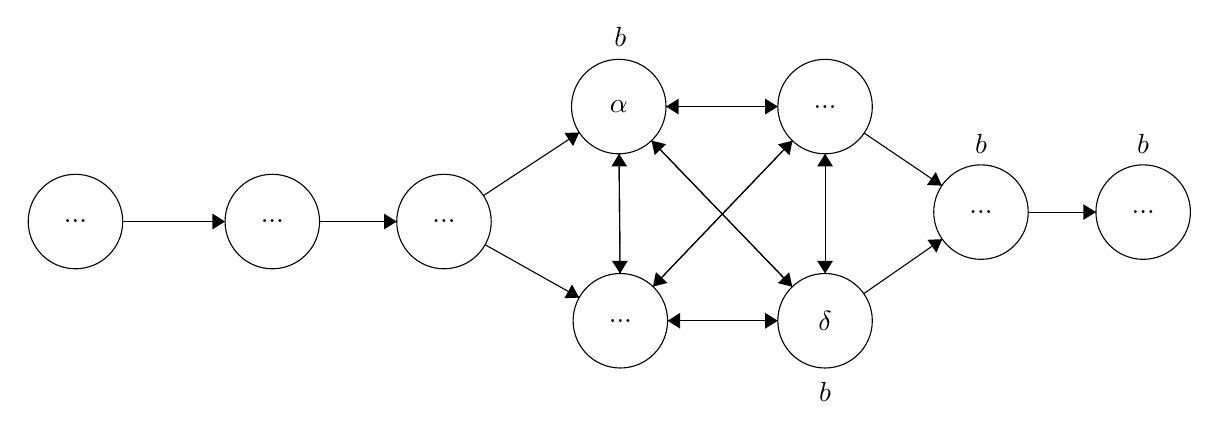
\begin{tikzpicture}[scale=0.2]  \tikzstyle{every node}+=[inner sep=0pt]  \draw [black] (6.9,-25) circle (3);  \draw (6.9,-25) node {$...$};  \draw [black] (19.4,-25) circle (3);  \draw (19.4,-25) node {$...$};  \draw [black] (30.3,-25) circle (3);  \draw (30.3,-25) node {$...$};  \draw [black] (41.4,-17.7) circle (3);  \draw (41.4,-17.7) node {$\alpha$};  \draw [black] (41.5,-31.3) circle (3);  \draw (41.5,-31.3) node {$...$};  \draw [black] (54.5,-17.7) circle (3); \draw (54.5,-17.7) node {$...$}; \draw [black] (54.5,-31.3) circle (3);  \draw (54.5,-31.3) node {$\delta$};  \draw [black] (64.4,-24.4) circle (3);  \draw (64.4,-24.4) node {$...$};  \draw [black] (74.7,-24.4) circle (3);  \draw (74.7,-24.4) node {$...$};  \draw (74.7,-20.1) node {$b$};  \draw (64.4,-20.1) node {$b$};  \draw (54.5,-35.8) node {\sout{$b$}};  \draw (41.5,-13.3) node {\sout{$\boxx{b}$}};  \draw [black] (9.9,-25) -- (16.4,-25);  \fill [black] (16.4,-25) -- (15.6,-24.5) -- (15.6,-25.5);  \draw [black] (22.4,-25) -- (27.3,-25);  \fill [black] (27.3,-25) -- (26.5,-24.5) -- (26.5,-25.5);  \draw [black] (32.81,-23.35) -- (38.89,-19.35);  \fill [black] (38.89,-19.35) -- (37.95,-19.37) -- (38.5,-20.21);  \draw [black] (32.91,-26.47) -- (38.89,-29.83);  \fill [black] (38.89,-29.83) -- (38.43,-29) -- (37.94,-29.87);  \draw [black] (41.48,-28.3) -- (41.42,-20.7);  \fill [black] (41.42,-20.7) -- (40.93,-21.5) -- (41.93,-21.5);  \draw [black] (41.42,-20.7) -- (41.48,-28.3);  \fill [black] (41.48,-28.3) -- (41.97,-27.5) -- (40.97,-27.5);  \draw [black] (51.5,-31.3) -- (44.5,-31.3);  \fill [black] (44.5,-31.3) -- (45.3,-31.8) -- (45.3,-30.8);  \draw [black] (44.5,-31.3) -- (51.5,-31.3);  \fill [black] (51.5,-31.3) -- (50.7,-30.8) -- (50.7,-31.8);  \draw [black] (54.5,-28.3) -- (54.5,-20.7); \fill [black] (54.5,-20.7) -- (54,-21.5) -- (55,-21.5); \draw [black] (54.5,-20.7) -- (54.5,-28.3); \fill [black] (54.5,-28.3) -- (55,-27.5) -- (54,-27.5);  \draw [black] (51.5,-17.7) -- (44.4,-17.7); \fill [black] (44.4,-17.7) -- (45.2,-18.2) -- (45.2,-17.2); \draw [black] (44.4,-17.7) -- (51.5,-17.7); \fill [black] (51.5,-17.7) -- (50.7,-17.2) -- (50.7,-18.2); \draw [black] (52.43,-19.87) -- (43.57,-29.13); \fill [black] (43.57,-29.13) -- (44.49,-28.9) -- (43.76,-28.21); \draw [black] (43.57,-29.13) -- (52.43,-19.87); \fill [black] (52.43,-19.87) -- (51.51,-20.1) -- (52.24,-20.79); \draw [black] (43.48,-19.86) -- (52.42,-29.14);  \fill [black] (52.42,-29.14) -- (52.22,-28.22) -- (51.5,-28.91);  \draw [black] (52.42,-29.14) -- (43.48,-19.86); \fill [black] (43.48,-19.86) -- (43.68,-20.78) -- (44.4,-20.09);  \draw [black] (56.96,-29.58) -- (61.94,-26.12);  \fill [black] (61.94,-26.12) -- (61,-26.16) -- (61.57,-26.98);  \draw [black] (56.98,-19.38) -- (61.92,-22.72); \fill [black] (61.92,-22.72) -- (61.53,-21.86) -- (60.97,-22.68); \draw [black] (67.4,-24.4) -- (71.7,-24.4);  \fill [black] (71.7,-24.4) -- (70.9,-23.9) -- (70.9,-24.9);  \end{tikzpicture}  \end{center}

allora, poiché la relazione è transitiva e connessa, abbiamo che

$\nonveraw{\mu}{\gamma}{\boxx b}$

e quindi, per questo possiamo dire che vale:

$\veraw{\mu}{\gamma}{\boxx b\implies b}$

per ogni cluster precedente a $C_{\alpha}$ e a $C_{\alpha}$stesso,
essendo falso il suo antecedente.

ma poiché in tutti i mondi successivi è vera b, allora in tutti i
mondi del modello è vera:

$\vera{\mu}{\boxx{(\boxx{b\implies b)}}}$

Però applicando a questo punto il modus ponens all'assioma Z e alla
precedente abbiamo che vale:

$\vera{\mu}{\diam{\boxx b}\implies\boxx b}$

Poiché per tutti i mondi dopo $C_{\alpha}$ è vera b, allora è vera
anche $\boxx b$

Ma allora in $\alpha$ vale:

$\veraw{\mu}{\alpha}{\diam{\boxx b}}$ 

poiché esistono dei mondi raggiungibili in cui è vera $\boxx b$

ma allora per Modus Ponens, è vale anche:

$\veraw{\mu}{\alpha}{\boxx b}$

Assurdo! La tesi allora deve essere valida.


\section{Altre logiche temporali}

Ci sono altre due logiche temporali interessanti:
\begin{enumerate}
\item K4DLDum, corretta e completa sul frame ($\omega$, $\leq$)
\item K4DLX corretta e completa sui frame ($\mathbb{Q}$,<) e ($\mathbb{R}$,<)
\end{enumerate}
Dove all'assioma Z vengono sostituiti rispettivamente:
\begin{itemize}
\item Dum: $\boxx{(\boa\implies a)\implies(\diam{\boa}\implies\boa)}$
\item X: $\boxx{\boa}\implies\boa$
\end{itemize}
Come si può notare non si può distinguere un tempo numerabile da un
tempo continuo.
